\section{Marco Teórico}

\subsection{Microcontrolador ATmega328P}

\begin{figure}[H]
  \centering
  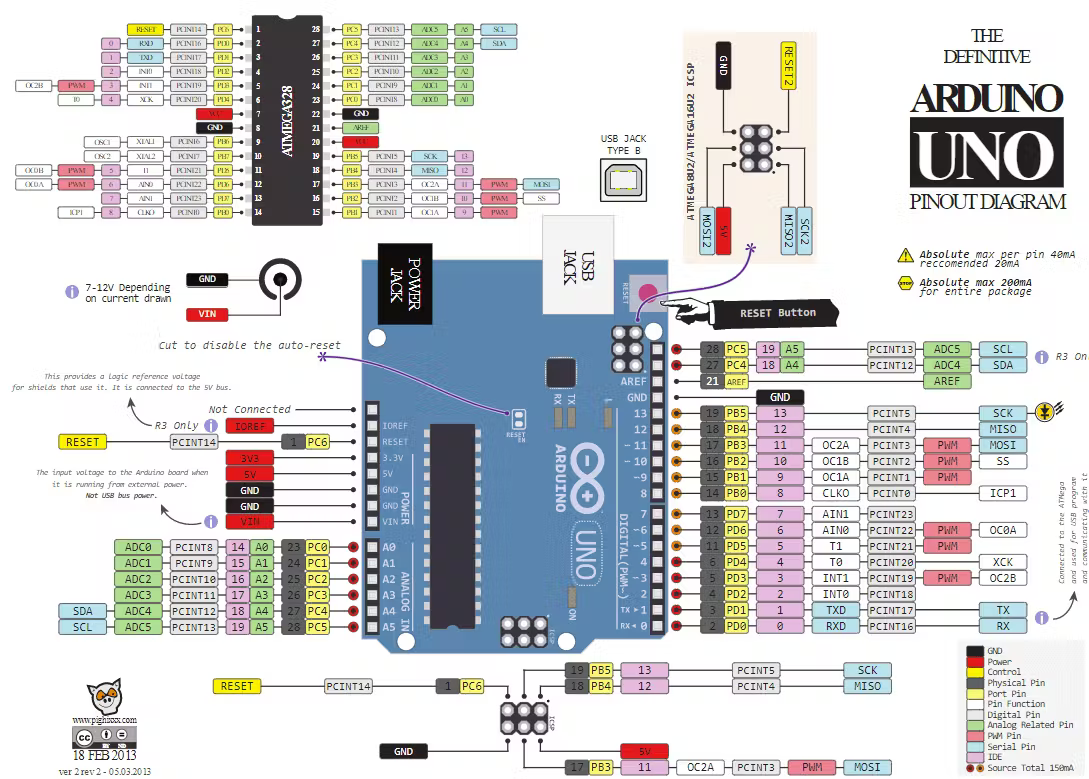
\includegraphics[width=\linewidth]{./Anexos/Full Arduino Pinout.png}
  \caption{Diagrama de pines del Arduino Uno. Fuente: \cite{arduino_uno_pinout}.}
  \label{fig:arduino-uno-pinout}
\end{figure}

\subsection{Registros de propósito general}

\subsection{Entradas y Salidas Digitales}
\begin{itemize}
    \item Concepto de GPIO.
    \item Uso de pulsadores como entradas digitales (debouncing si es necesario).
    \item Uso de LEDs como indicadores de estado.
\end{itemize}


\subsection{Stack Pointer}

Incialización del Stack Pointer:

\begin{verbatim}
RESET:
    cli ldi r16, high(RAMEND)
    out SPH, r16
    ldi r16, low(RAMEND)
    out SPL, r16 sei
    ; ...
\end{verbatim}

Usos del Stack Pointer: rcall, call, interrupciones
preservacion de datos entre subrutinas e ISRs

\begin{verbatim}
MI_ISR:
    push r16
    out r16, SREG
    push r16
    ; ... 
    pop r16
    in SREG, r16
    push r16
    reti
\end{verbatim}

\subsection{Timers}
El atmega328p tiene 3 timers diferentes: Timer 0, Timer 1, y Timer 2.

Timer 0 y 2 son de 8 bits
Timer 1 es de 16 bits (puede contar más)

La ecuacion para calcular el tiempo del timer es la siguiente.

\begin{equation}
    \frac{(2^{k} - C_{\text{inicio}})\cdot \text{Prescaler}}{f_{\text{contador}}} = t_{\text{deseado}}
\end{equation}

Esta ecuación determina el tiempo que le tomaría al contador hacer un desbordamiento (overflow) en base a la frecuencia a la cantidad de bits del contador (k), la frecuencia de trabajo del microcontrolador, el tiempo o conteo con el que se inicie el contador, y el prescaler con el que esté configurado.

El prescaler del Temporizador 1 es configurado a través del registro TCCR1B el cual posee la siguiente configuración:

\begin{figure}[H]
  \centering
  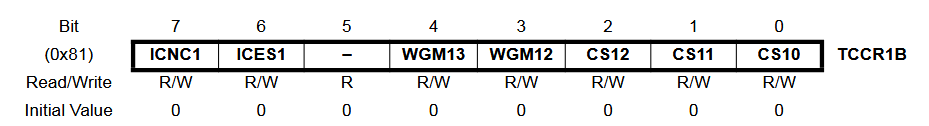
\includegraphics[width=\linewidth]{./Anexos/Marco Teorico/Timers/TCCR1B.png}
  \caption{Registro de control B (TCCR1B) para Timer/Counter1. Fuente: hoja de datos del ATmega328P\@\cite{atmega328p_datasheet}.}
  \label{fig:TCCR1B}
\end{figure}

Los bits CS12 CS11 y CS10 configuran el prescaler del timer conforme a la siguiente tabla: 

\begin{figure}[H]
  \centering
  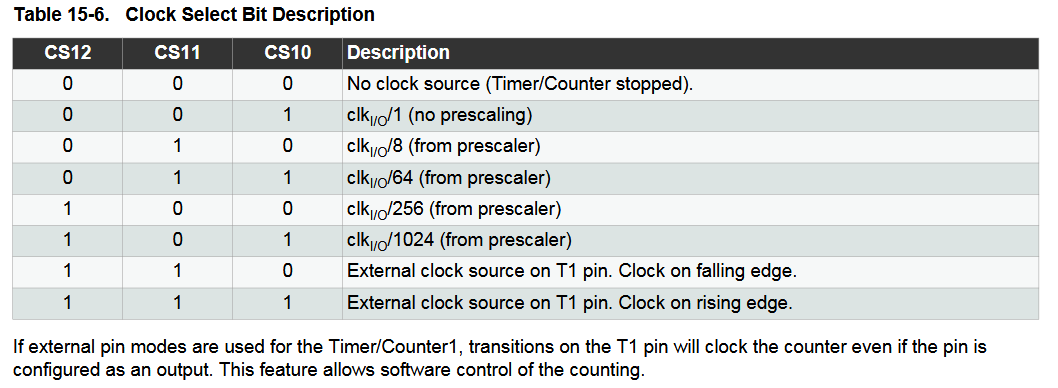
\includegraphics[width=\linewidth]{./Anexos/Marco Teorico/Timers/Prescaler Table.png}
  \caption{Clock Select (CS12:0) opciones de prescaler para Timer/Counter1. Fuente: hoja de datos del ATmega328P\@\cite{atmega328p_datasheet}.}
  \label{fig:prescaler-table}
\end{figure}


El máximo valor de tiempo que admite el Timer 1 (de 16 bits) con el prescaler de 1024 es de 4.19 segundos (aproximadamente). Para valores más grande de delay será necesario crear un contador de overflow aparte utilizando registros de uso general o SRAM

Este es un ejemplo de inicialización de timer 1 para un overflow de 1s

\begin{verbatim}
ldi r16, 0b101       sts TCCR1B, r16
ldi r16, HIGH(49911) sts TCNT1H, r16
ldi r16, LOW(49911)  sts TCNT1L, r16 
\end{verbatim}

El primer registro (TCCR1B) determina el prescaler del reloj (según la figura\ \ref{fig:prescaler-table})

Utilizando la tabla de vectores de interrupcion que se muestra en la figura\ \ref{fig:interrupt-vectors} se mapea el vector de interrupción con la etiqueta del ISR correspondiente:

\begin{verbatim}
.org 0x001A rjmp TIMER1_OVF_ISR

TIMER1_OVF_ISR:
    push r16
    out r16, SREG
    push r16
    ; ... 
    pop r16
    in SREG, r16
    push r16
    reti
\end{verbatim}

\begin{figure}[H]
  \centering
  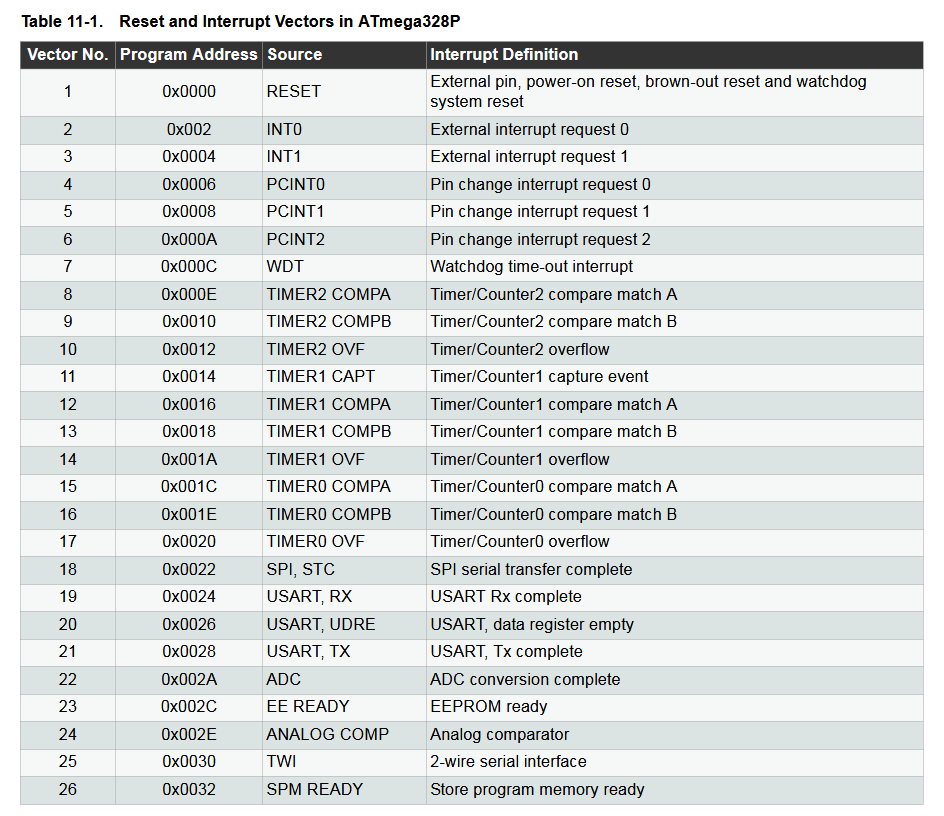
\includegraphics[width=\linewidth]{\detokenize{./Anexos/Marco Teorico/Interrupt Vectors.png}}
  \caption{Vectores de interrupciones en el ATmega328P. Fuente: hoja de datos del ATmega328P\@\cite{atmega328p_datasheet}.}
  \label{fig:interrupt-vectors}
\end{figure}

El mismo proceso puede ser aplicado para configurar los otros dos Timers.

\subsection{Interrupciones externas}

   \begin{figure}[H]
    \centering
    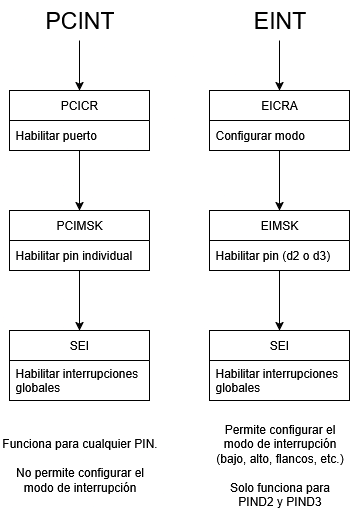
\includegraphics[width=0.7\linewidth]{./Anexos/Marco Teorico/External Interrupts/Interrupt diagram.png}
    \caption{Flujo de configuración de interrupciones exeternas. Fuente: Elaboración própia.}
    \label{fig:InterruptDiagram}
    \end{figure}


    \subsubsection{EINT}
    Interrupciones externas 

    \begin{figure}[H]
    \centering
    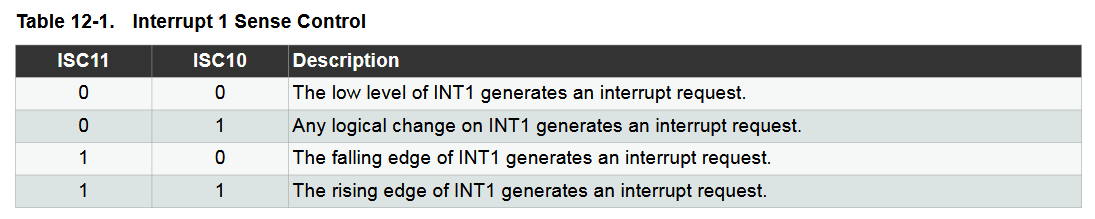
\includegraphics[width=\linewidth]{./Anexos/Marco Teorico/External Interrupts/EICRA table.png}
    \caption{Tabla de configuraciones para EICRA. Fuente: hoja de datos del ATmega328P\@\cite{atmega328p_datasheet}.}
    \label{fig:EICRA-table}
    \end{figure}

    \begin{figure}[H]
    \centering
    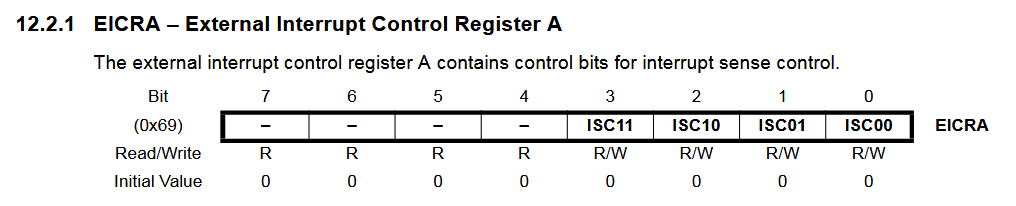
\includegraphics[width=\linewidth]{./Anexos/Marco Teorico/External Interrupts/EICRA.png}
    \caption{Registro de configucación de interrupciones externas EICRA. Fuente: hoja de datos del ATmega328P\@\cite{atmega328p_datasheet}.}
    \label{fig:EICRA}
    \end{figure}

    \begin{figure}[H]
    \centering
    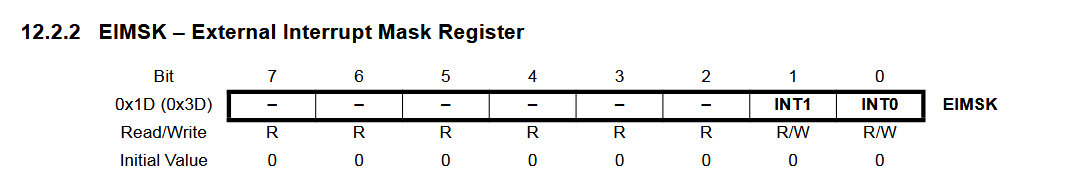
\includegraphics[width=\linewidth]{./Anexos/Marco Teorico/External Interrupts/EIMSK.png}
    \caption{Registro de configucación de máscaras de interrupciones externas EICRA. Fuente: hoja de datos del ATmega328P\@\cite{atmega328p_datasheet}.}
    \label{fig:EIMSK}
    \end{figure}

    \subsubsection{PCINT}
    Interrupciones por cambio en PIN


    \begin{figure}[H]
    \centering
    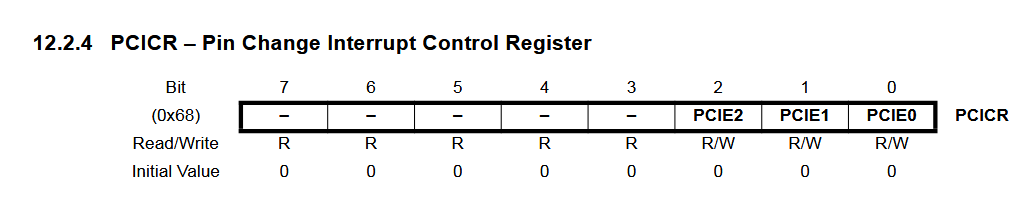
\includegraphics[width=\linewidth]{./Anexos/Marco Teorico/External Interrupts/PCICR.png}
    \caption{Registro de configucación interrupciones PCICR (PCINT). Fuente: hoja de datos del ATmega328P\@\cite{atmega328p_datasheet}.}
    \label{fig:PCICR}
    \end{figure}

    \begin{figure}[H]
    \centering
    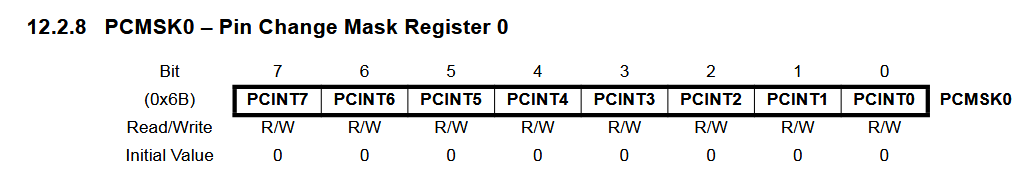
\includegraphics[width=\linewidth]{./Anexos/Marco Teorico/External Interrupts/PCMSK.png}
    \caption{Registro de configucación de mascara de pines para interrupciones PCIMSK0 (PCINT). Fuente: hoja de datos del ATmega328P\@\cite{atmega328p_datasheet}.}
    \label{fig:PCIMSK}
    \end{figure}



\subsection{SRAM}

\begin{verbatim}
.dseg
variable: byte 1  
arreglo: byte 100
\end{verbatim}

Usando dseg se puede reservar espacio en memoria la SRAM para utilizarlo luego. Posteriormete con ``variable'' podremos leer o escribir el valor guardado con ``lds'' o ``sts'' respectivamente. O incluse se podría utilizar un puntero (X, Y, Z) para acceder a un lugar en memoria de manera iterativa donde quisieramos guardar múltiples valores subsecuentes (como un arreglo). 

Nota: Existen 2kb de memoria RAM, el stack pointer vive dentro de la RAM así que uno debe ser precabido con el uso excesivo de este recurso.

\subsection{FLASH}

\begin{verbatim}
.cseg
.org 0x300 TABLA:
    .db 0xFF, 0x30, 0x30, 0xFF
\end{verbatim}

Utilizando .cseg y una dirección segura como 0x300 para guardar datos, se puede utilizar la misma memoria FLASH para guardar datos constantes como LUTs, fotogramas, cadenas de texto, etc. Estos datos no pueden ser modificados, pero existen 32kb de espacio en memoria FLASH para guardar información, por lo que es menos limitante que la SRAM (2kb)

Para acceder a datos guardados en program memoria del programa (FLASH) se puede hacer haciendo uso del puntero Z y la instrucción ``lpm'':

\begin{verbatim}
GET_DATA:
    ldi ZH, high(TABLA<<1)
    ldi ZL, low(TABLA<<1)
    lpm r16, Z+
    ret
\end{verbatim}

Se carga la dirección a Z cargando las partes bajas y altas de la dirección a ZL y ZH respectivamente. En los AVR  ``clásicos'' (como el ATmega328P), las etiquetas en memoria de programa (.cseg) están en direcciones de palabra (cada instrucción ocupa 16 bits), pero la instrucción LPM usa una dirección en bytes en el registro Z. Por eso se hace $<$$<$ 1 (multiplicar por 2): convierte la dirección en palabras de la etiqueta a dirección en bytes para LPM. Y ``Z+'' indica que luego de realizar lpm, se incremente en 1 el puntero ``Z''

\begin{figure}[H]
  \centering
  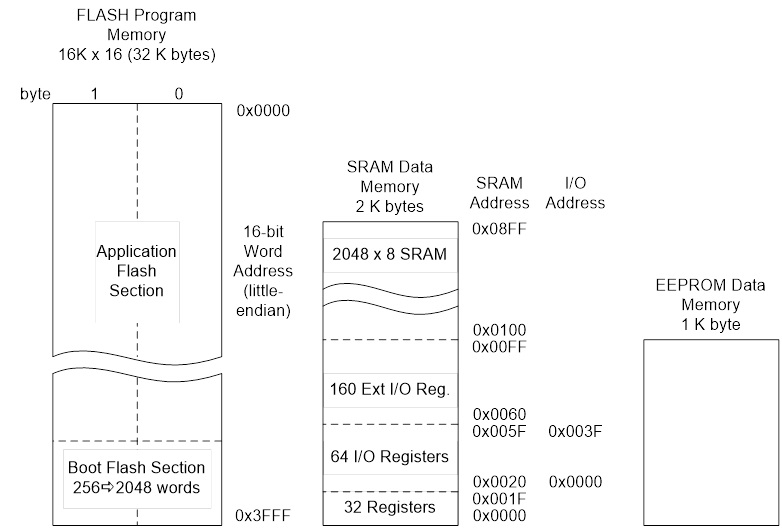
\includegraphics[width=\linewidth]{./Anexos/Memory Map.jpg}
  \caption{Mapa de memoria y espacios de direcciones en AVR de 8 bits. Fuente: \cite{arxterra_avr_addressing_modes}.}
  \label{fig:avr-memory-map}
\end{figure}


\subsection{USART Asíncrono}
    \subsubsection{Inicialización}
    \begin{verbatim}
    .equ _F_CPU = 16000000
    .equ _BAUD = 9600
    .equ _BPS = (_F_CPU/16/_BAUD) - 1

    .org 0x0024 rjmp USART_RX_ISR
    
    RESET:
    ; Configurar baudios
    sts UBRR0H, high(_BPS)
    sts UBRR0L, low(_BPS)

    ; Habilitar: receptor, transmisor
    ; e interrupciones por RX
    ldi r16, 0b10011000
    sts UCSR0B,r16

    ; Establecer formato:
    ; 8 data bits, 2 stop bits
    ldi r16, (1<<USBS0)|(3<<UCSZ00)
    sts UCSR0C,r16

    sei
    \end{verbatim}
    \subsubsection{Transmisión}
    \begin{verbatim}
    ldi r16, 0x3f ; Cargar r16 
    sts  UDR0, r16 ; Transmitir
    \end{verbatim}
    \subsubsection{Recepción}

    \begin{verbatim}
    USART_RX_ISR:
    push r16 
    in r16, SREG 
    push r16 

    ; Datos recibidos en r16
    lds r16, UDR0
    ; ...

    pop r16
    out SREG, r16
    pop r16	
    reti
    \end{verbatim}
    \subsubsection{USART con Ring Buffer}


    \paragraph*{Inicialización}
    \begin{verbatim}
    .dseg ; Ring buffer ram alocation
    tx_buffer: .byte TX_BUF_SIZE  
    tx_head:   .byte 1            
    tx_tail:   .byte 1           

    .cseg
    .equ TX_BUF_SIZE = 256
    .equ TX_BUF_MASK = TX_BUF_SIZE - 1

    .equ _F_CPU = 16000000
    .equ _BAUD = 57600 
    .equ _BPS = (_F_CPU/16/_BAUD) - 1
    
    ; Recieved USART data
    .org 0x0024 rjmp USART_RX_ISR	
    ; USART Data register clear
    .org 0x0026 rjmp USART_UDRE_ISR 

    RESET:
    clr r1

    ; Stack 
    ldi r16, high(RAMEND) out SPH, r16
    ldi r16, low(RAMEND)  out SPL, r16

    ; Init USART
    ldi r16, low(_BPS)
    ldi r17, high(_BPS)
    rcall USART_INIT

    sei
    ; ...

    USART_INIT:	
    sts  tx_head, r1
    sts  tx_tail, r1

    sts UBRR0H, r17
    sts UBRR0L, r16

    ldi r16, 0b10011000
    sts UCSR0B,r16

    ldi r16, (1<<USBS0)|(3<<UCSZ00)
    sts UCSR0C,r16
    ret
    \end{verbatim}


    \paragraph*{Subrutina USART WRITE BYTE}
    \begin{verbatim}
    USART_WRITE_BYTE:
    push r17
    push r18
    push r19
    push ZH
    push ZL

    ; head/tail
    lds  r17, tx_head
    lds  r18, tx_tail

    ; r16 -> next = (head + 1) & MASK 
    mov  r19, r17
    inc  r19
    andi r19, TX_BUF_MASK 
    ; Clamping:
    ; Con 256 es 0xFF: no cambia, 
    ; pero deja claro el patrón

    wait_space:
    ; full? next == tail
    lds  r18, tx_tail
    cp   r19, r18
    breq wait_space

    have_space:
    ; Z -> Cabeza de buffer
    ldi  ZL, low(tx_buffer)
    ldi  ZH, high(tx_buffer)
    add  ZL, r17 
    adc  ZH, r1

    st   Z, r16 ; Guardar en buffer

    ; Cabeza = next
    sts  tx_head, r19

    ; Habilitar interrupcion UDRE
    ; así el ISR comienza/continúa 
    ; drenando el buffer
    cli
    lds  r18, UCSR0B
    ori  r18, (1<<UDRIE0)
    sts  UCSR0B, r18
    sei

    pop  ZL
    pop  ZH
    pop  r19
    pop  r18
    pop  r17
    ret
    \end{verbatim}


    \paragraph*{Interrución USART UDRE ISR}
    \begin{verbatim}
    USART_UDRE_ISR:
    push r16
    in   r16, SREG
    push r16
    push r17
    push r18
    push r20
    push ZH
    push ZL

    ; r17 = head, r18 = tail
    lds  r17, tx_head
    lds  r18, tx_tail

    ; buffer vacío? head == tail
    cp   r17, r18
    brne usart_udre_send

    ; vacío: deshabilitar UDRIE0
    lds  r20, UCSR0B
    andi r20, ~(1<<UDRIE0)
    sts  UCSR0B, r20
    rjmp usart_udre_exit

    usart_udre_send:
    ; Z -> Cola de buffer
    ldi  ZL, low(tx_buffer)
    ldi  ZH, high(tx_buffer)
    add  ZL, r18
    adc  ZH, r1 

    ; Transmitir byte
    ld   r16, Z
    sts  UDR0, r16

    ; cola = (cola + 1)
    inc  r18                
    andi r18, TX_BUF_MASK 
    ; Clamping:
    ; Con 256 es 0xFF: no cambia, 
    ; pero deja claro el patrón

    sts  tx_tail, r18

    usart_udre_exit:
    pop  ZL
    pop  ZH
    pop  r20
    pop  r18
    pop  r17
    pop  r16
    out  SREG, r16
    pop  r16
    reti
    \end{verbatim}

    
    \paragraph*{Interrución USART RX ISR}
    \begin{verbatim}
    USART_RX_ISR:
    push r16 
    in r16, SREG
    push r16

    lds r16, UDR0 
    ; ...

    pop r16
    out SREG, r16
    pop r16
    reti
    \end{verbatim}
    



\subsection{Automatización y Máquinas de Estado}
\begin{itemize}
    \item Qué es una máquina de estados finitos.
    \item Cómo se representan los estados y transiciones en un proceso automatizado (ejemplo: espera → alimentación → posicionado → punzonado → descarga → fin de ciclo).
\end{itemize}


\subsection{Control de Procesos con Cinta Transportadora y Punzonadora}
\begin{itemize}
    \item Principios básicos de una cinta transportadora en automatización.
    \item Funcionamiento de un actuador lineal/solenoide como punzón.
    \item Diferentes modos de operación según carga (ligera, media, pesada).
\end{itemize}


\subsection{Comunicación Serial (USART/UART)}
\begin{itemize}
    \item Definición y funcionamiento de UART.
    \item Ejemplos de comandos y monitoreo remoto.
    \item Aplicaciones en sistemas embebidos para interacción con el usuario o con PC.
\end{itemize}


\subsection{Conversión Digital-Analógica (DAC R-2R)}
\begin{itemize}
    \item Concepto de DAC y su importancia.\vspace{0.5em}
    
    Un DAC (Digital to Analog Converter) es un dispositivo o técnica que permite transformar valores digitales (códigos binarios) en señales analógicas (tensiones o corrientes continuas y variables en el tiempo). Su importancia radica en que la mayoría de los sistemas electrónicos trabajan de manera digital, pero el mundo físico es analógico: audio, imágenes, señales de control de motores, etc.
    
    En pocas palabras, el DAC es el “puente” entre lo digital y lo analógico.\vspace{1em}

    \item Arreglo de resistencias R-2R.\vspace{0.5em}

    El arreglo R-2R es una red de resistencias que se usa mucho para construir DACs simples y económicos. Se compone unicamente de dos valores de resistencias: una de valor R y otra de valor 2R, que se repiten en forma de escalera.
    
    Cada bit de nel número digital controla un interruptor (o transistor) que conecta la red a una referencia de tensión (Vref) o a tierra. Gracias a la proporción entre Ry 2R, la red genera tenciones que corresponden al valor binario aplicado.
    
    La ventaja del arreglo R-2R es que es fácil de implementar, no requiere de resistencias con muchos valores distintos, y mantienen una buena presición.\vspace{1em}
    
    \item Uso de una Look-Up Table (LUT) para generar señales analógicas periódicas.\vspace{0.5em}
    
    Una Look-up Table (LUT) es básicamente una tabla de valores precargada en la memoria que representa una señal digitalizada (por ejemplo, una onda seno). En lugar de calcular cada valor de la función en tiempo real, el monitor solo "lee" la tabla en orden y envía los valores a un puerto o a un DAC.
    
    Cuando esos valores se aplican de manera periódica y con la velocidad adecuada, en la salida se reconstruye una señal analógica periodica.
    
    El uso de una LUT simplifica mucho la generación de señales, por que evita cálculos complejos y garantiza que la forma de onda siempre tenga la misma calidad.\vspace{1em}
\end{itemize}


\subsection{Matrices de LEDs}
\begin{itemize}
    \item Principio de funcionamiento de una matriz de LEDs.
    \item Multiplexado y desplazamiento de mensajes.
    \item Ejemplo de uso en displays.
\end{itemize}


\subsection{Plotter y Control de Movimiento}
\begin{itemize}
    \item Concepto de plotter y su uso en ingeniería.
    \item Control de motores paso a paso o conmutados mediante relés/MOSFETs.
    \item Señales de control enviadas desde el microcontrolador a un PLC.
\end{itemize}
